\documentclass{sig-alternate-05-2015}
\usepackage{subfigure}
\usepackage{balance}
\usepackage{multirow}
\usepackage{color}
\usepackage{chngpage}
\usepackage{url}
\usepackage{amsmath}

\newtheorem{theorem}{Theorem}[section]

\newcommand{\para}[1]{{\vspace{2pt} \bf \noindent #1 \hspace{8pt}}}

\newenvironment{packed_itemize}{
\begin{itemize}

}{\end{itemize}}


\makeatletter
\def\@copyrightspace{\relax}
\makeatother

\begin{document}

\title{Markov Chain Monte Carlo}
\subtitle{Introduction, Comparison \& Analysis}
\author{
    \alignauthor Tzu-Heng Lin, 2014011054, W42\\
    \affaddr{Department of Electronic Engineering, Tsinghua
      University, Beijing, China\\}
    \email{lzhbrian@gmail.com}
}


\maketitle
\begin{abstract}
Markov Chain Monte Carlo (MCMC) is a technique to make an estimation of a statistic by simulation in a complex model. Restricted Bolztmann Machine(RBM) is a crucial model in the field of Machine Learning. However, training a large RBM model will include intractable computation of the partition functions, i.e.Z($\theta$). This problem has aroused interest in the work of estimation using a MCMC methods.
In this paper, we first conduct Metropolis-Hastings Algorithm, one of the most prevalent sampling methods, and analyze its correctness \& performance, along with the choice of the accepting rate. We then implement three algorithms: TAP, AIS, RTS, to estimate partition functions of an RBM model. Our work not only give an introduction about the available algorithms, but systematically compare the performance \& difference between them. We seek to provide an overall view in the field of MCMC.
\end{abstract}




%
%  Use this command to print the description
%
\printccsdesc

%!TEX root = head-full.tex


%  On one hand, the development of the broadband services greatly
% improves the user experience of 

\section{Introduction} \label{sec:introduction}

\para{Markov Chain}
A Markov Chain is a special stochastic process in which the current state only depends on its previous state, we call this property the Markov property or memorylessness. i.e.
\begin{equation}
P(X_{t+1}=x|X_t, X_{t-1}, \cdots) =P(X_{t+1}=x|X_t)
\end{equation}

Given a Markov Chain, if a vector $\pi$, has the property:
\begin{equation}
\pi=\pi P
\end{equation}
then we call $\pi$ the stationary distribution, it denotes the final state distribution of the stochastic process in a Markov Chain.

Markov Chain has a wide application in many fields in the real world, such as social science\cite{acemoglu2011political}, econmics \& finance\cite{hamilton1989new} and of course, computer science\cite{page1999pagerank}, etc.

\para{Markov Chain Monte Carlo}
If we are given a probability distribution $p(x)$, it would be a great thing if we could generate some samples of it by a simple method, so here comes the Markov Chain Monte Carlo(MCMC) method. If we could construct a Markov Chain which its stationary distribution $\pi$ just equals to $p(x)$, then we could use this Markov Chain to sample from this distribution $p(x)$. And this is the main idea of MCMC.

In this paper, we implement the Metropolis-Hastings Algorithm\cite{metropolis1953equation,hastings1970monte}, which is one of the most widely used sampling method. We also deal with the accepting rate, which I will introduce later, for previous work\cite{roberts1997weak} have shown that the accepting rate may influence the result of the experiment and there is theoretical support in choosing an optimal accepting rate.

\para{Restricted Boltzmann Machine}
A Restricted Bolztmann Machine (RBM)\cite{mcclelland1987parallel} is a significant work bringing hypothesis in statistical physics to computer science. By stacking several layers of RBM, we will get a fundamental model, Deep Belief Network\cite{hinton2006reducing}, in the field of Deep Learning, which is nowadays the hottest class of algorithms used in Machine Learning.

\para{Estimating Partition functions} 
In the process of training an RBM, however, will include incontractable computation of the partition function. When the model grows large, the complexity of this work will be incompletable. The good news is, several researches have shown that there are ways to avoid this by using an MCMC approach instead, to estimate it.

In this paper, we implement three prevalent MCMC methods of estimating a partition function, Thouless-Anderson-Palmer Sampling(TAP)\cite{gabrie2015training}, Annealed Importance Sampling (AIS)\cite{neal2001annealed,salakhutdinov2009learning}, Rao-Blackwellized Tempered Sampling(RTS)\cite{carlson2016partition}, respectively, and give an overall comparison on the theory \& performance between them.





%!TEX root = head-full.tex

\section{Metropolis-Hastings} \label{sec:metropolis_hastings}
Metropolis Hastings(MH) Algorithm

\subsection{Algorithm\protect\footnote{Available at \protect\url{https://github.com/lzhbrian/MCMC/blob/master/metropolis_hastings/metropolis_hasting.R} in Matlab}}

\subsubsection{Detailed Balance Condition}

\subsubsection{General Case}

\subsubsection{Symmetric Case}




\subsection{Sampling Results}
In our work, we use an example of a bivariate Normal distribution, with
$$ \mu = \left( \begin{array}{ccc}
5 \\
10 \end{array} \right), 
\Sigma = \left( \begin{array}{ccc}
1 & 1\\
1 & 4\end{array} \right)$$

By theoretical computation, we can easily compute the the pearson correlation between the two dimensional value is 0.5.
$$ \rho = 0.5 $$

We then generate 10,000 samples using the MH algorithm, setting the standard deviation of proposal to 3.0. We can see from the result (Figure~\ref{fig:sample_result}) that we have derived 10,000 sampled points with pearson correlation = 0.5, which matches the theoretical value.

\begin{figure}[t]
\vspace{-0.5in}
  	\centering
  	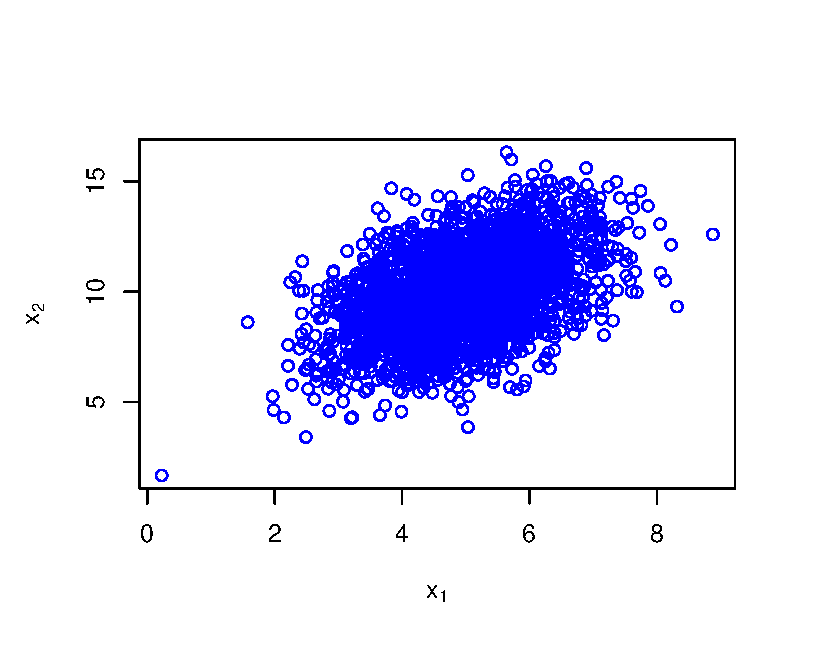
\includegraphics[width=0.4\textwidth]{figure/sample_result.eps}
\vspace{-0.2in}
	\caption{Sampling result of 10,000 points \protect\\ correlation = 0.500873 , set sd.T = 3.0}
	\label{fig:sample_result}
\end{figure}


\subsection{Performance Analysis}
MH algorithm is an effective MCMC method for many diverse problems. However, its efficiency depends crucially on the selection of the proposal density. With the proposal jump size being small, the accepting rate would be very low and eventually stick to only one point(eg. the initial point); When the proposal jump size is too big, the accepting rate would be too high. 

Roberts et al. have shown in previous work\cite{roberts1997weak} that the optimal accepting rate of the MH algorithm should approximately be at 0.234 for the case of an N-dimensional Gaussian target distribution. We test the accepting rates in different proposal jump size(Figure~\ref{fig:acc_sdt}) and find that the optimal value should be at appoximately 3.0 to acquire a model with accepting rate being close to 0.234.

\begin{figure}[t]
\vspace{-0.5in}
  	\centering
  	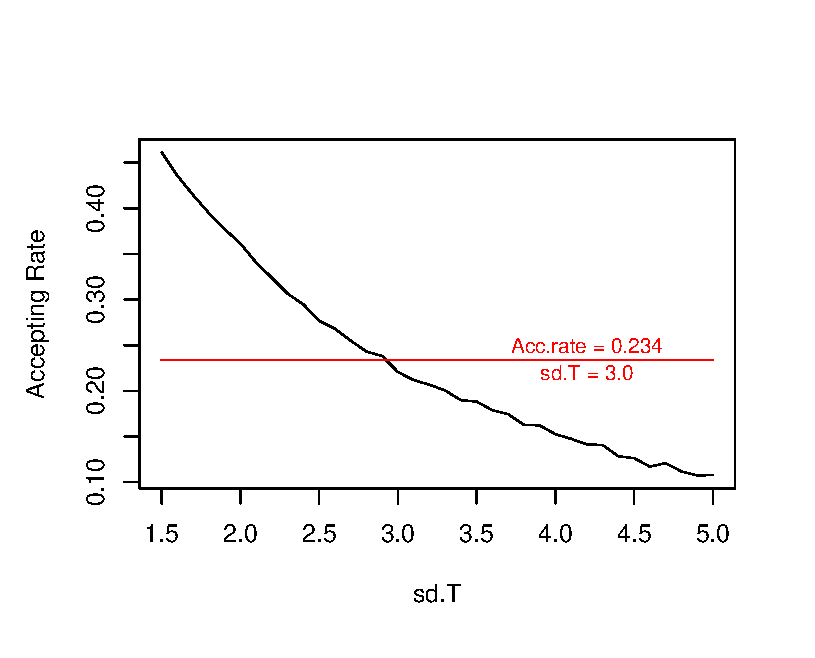
\includegraphics[width=0.4\textwidth]{figure/acc_sdt.eps}
\vspace{-0.2in}
	\caption{Accepting rate on different proposal jump size.}
	\label{fig:acc_sdt}
\end{figure}

\subsection{Gibbs Sampling}
For a high dimensional condition, because of the limit of accepting rate, the efficiency of MH algorithm is not satisfying, so many would switch to Gibbs Sampling Algorithm.

Gibbs Sampling is a special case of Metropolis Hastings Algorithm, by letting the accepting rate = 1, we will get a Gibbs Sampler. As the length \& time limit, we will not specify more here.







%!TEX root = head-full.tex

\section{Partition Function Estimation} \label{sec:rbm}



\subsection{Restricted Bolztmann Machine}
Restricted Bolzmann Machine ...
However, calculating partition functions has always been a ...



\subsection{Algorithms}

\subsubsection{Thouless-Anderson-Palmer Sampling\protect\footnote{Available at \protect\url{https://github.com/lzhbrian/MCMC/blob/master/rbm/TAP.m} in Matlab}}



\subsubsection{Annealed Importance Sampling\protect\footnote{Available at \protect\url{https://github.com/lzhbrian/MCMC/blob/master/rbm/AIS.m} in Matlab}}
\subsubsection{Rao-Blackwellized Tempered Sampling\protect\footnote{Available at \protect\url{https://github.com/lzhbrian/MCMC/blob/master/rbm/RTS.m} in Matlab}}
\subsubsection{Other method}
There are many other methods which can also estimate the partition functions. Such as Self-adjusted mixture sampling(SAMS)\cite{tan2015optimally} proposed a method to estimate multiple partition functions together to improve the efficiency. As the length \& time limit, we only implement 3 methods here in this paper.


\subsection{Estimating Results}



\subsection{Performance Analysis}
\subsubsection{}





% Conclusion

%!TEX root = head-full.tex

\section{Related Work} \label{sec:relatedwork}

% the study of video access behavior

\para{Video Access Behavior.}These works usually focus on one single system, and their analysis is also limited to a specific context. In contrast, our work collects a dataset of video viewing behaviors across six major video providers with contexts such as VoD, IPTV, live streaming. This allows us to understand user migratory patterns across content providers. \cite{roberts1997weak} analyze the influence of video stream quality on user behavior from multiple CPs using quasi-experimental designs, but they do not have an in-depth study of characterizing migration behaviors.  \cite{metropolis1953equation}\cite{hastings1970monte}


\section{Conclusion} \label{sec:conclusion}
In this paper, we discuss about the Markov Chain Monte Carlo method which are now undoubtedly one of the most important sampling methods.

We comprehensively introduce the concept of Metropolis-Hastings Algorithm and conduct an experiment to verify its correctness. We also make some analysis about how accepting rate would interfere the sampling result.

We systematically compare three methods of partition function estimationm which are crucial works in training a Restricted Bolztmann Machine or a Deep Belief Network. 

As future work, we would like to join more methods to the comparison and if could, propose some improvement to the algorithms available.


\renewcommand{\baselinestretch}{1.1}
\balance

\small

% Acknowledgement
\section{Acknowledgement} \label{sec:acknowledgement}
I would like to thank Yubo Chen, Liren Yu, Yuanxin Zhang, XueChao Wang, Changran Hu, for the discussion with me on the algorithms. Without them, I wouldn't have the possibility to accomplish this work in such a short time. This paper is a project of Stochastic Process Course in Tsinghua University, taught by Prof. Zhijian Ou.

% Reference
\bibliographystyle{abbrv}
\bibliography{ref}

	

\end{document}

